\section{Numerical verification and solution limits}
\label{sec:verification}
% P:verification-01
Numerical verification isolates errors in equations, closures, derivatives and solved-state transport from the physical discrepancies in Section~\ref{sec:physical}.
Table~\ref{tab:verification} summarizes representative checks with their reference and unit.
Cross-code comparisons use matched parameters, equations and constants; finite-difference comparisons use declared directions and step refinement on the same smooth branch.
An observed code difference without an independent reference is not automatically an error of one code.
Unless stated otherwise, the comparisons use FeOs~0.10.1, Clapeyron.jl~0.6.29 and teqp~0.23.2; the five-code propane comparison uses the surveyed source versions in Table~\ref{tab:software}.

\begin{table}[pos=htbp]
\centering\small
\caption{Numerical verification on the stated populations. Bounds are rounded outward. Ratios to a criterion are dimensionless and do not represent physical model errors.}
\label{tab:verification}
\begin{tabularx}{\linewidth}{@{}p{0.37\linewidth}p{0.29\linewidth}X@{}}
\toprule
Quantity / population & Reference & Maximum difference or ratio \\
\midrule
Propane saturation pressure, 300~K & Five matched codes & $1.10\times10^{-9}$ relative \\
Propane critical candidate & FeOs; teqp & $8.3\times10^{-11}$; $8.3\times10^{-15}$ relative \\
First solved-state actions, bubble and liquid split & Clapeyron implicit derivatives & $3.40\times10^{-10}$ relative \\
Electrolyte liquid compositions, 8 feeds & Matched constant-permittivity Clapeyron flash & $4.62\times10^{-9}$ mole fraction \\
Direct Born term, aqueous NaCl & Matched constants, Clapeyron; FeOs & $3.41\times10^{-16}$; $8.21\times10^{-12}$ relative \\
Dipole contribution, 8 states & teqp & $10^{-15}$ relative \\
Pressure-specified caloric actions, 36 comparisons & Refined differences & 0.34 of criterion \\
Selected second / third solved actions & Refined lower actions; analytic isomerization & $5.92\times10^{-4}$ / $2.45\times10^{-4}$ of criterion \\
Electrolyte fitting columns, 3\,167 & Refined differences & 0.0145 of allowance \\
Two-reaction ionic extraction feed actions & Finer of two central-difference steps & $3.52\times10^{-6}$ relative \\
Selected density roots, 704 requests & Frozen / separate scan & $1.56\times10^{-11}$ / $1.60\times10^{-11}$ relative \\
Same density requests, pressure closure & Defining pressure equation & $2.19\times10^{-13}$ reduced residual \\
Manufactured reacting caloric comparisons & Identities, refined differences, quadrature & 0.0952 of criterion among numerical ratios \\
Manufactured least-squares / minimax coordinates & Known parameters / analytic optimality & $7.35\times10^{-11}$ / $6.01\times10^{-11}$ absolute \\
\bottomrule
\end{tabularx}
\end{table}

\subsection{Shared equations across independent implementations}
\label{sec:cross-code}
% P:verification-02
Propane saturation at 300~K with Gross--Sadowski parameters~\citep{Gross2001} gives a common case for this package, FeOs, Clapeyron.jl, teqp and ThermoPack.
The pressure agrees within the bound in Table~\ref{tab:verification}; representative numerical values appear in the Supporting Information for independent implementation checks.
The critical and neutral bubble/dew comparisons in the full envelope gallery are discrete numerical comparisons, separate from the native continuation line.
Pressure--enthalpy and pressure--entropy comparisons with FeOs use the same manufactured ideal-gas thermal records and common caloric increments, avoiding a false comparison between different reference enthalpies.
The shared-model checks do not assess experimental caloric accuracy.

% P:verification-03
A direct Born comparison for aqueous NaCl matches electrostatic constants before evaluating the code difference.
The remaining differences are much smaller than the discrepancy obtained with unmatched constants.
The optional dipole term likewise agrees with teqp on selected fixed neutral states~\citep{Gross2006,bellImplementingEquationState2022}.
The corrected solvation-shell Born term and ion-suppression relation have derivative/identity checks but no independent same-equation value implementation in this comparison.
That gap is distinct from the measured-data errors of those parameterizations.

% P:verification-04
For the eight water/ethanol/isobutanol/NaCl feeds at 293.15~K and 100~kPa, constant permittivity and the direct Born term define a deliberately matched electrolyte model.
Clapeyron.jl then reproduces the package's phase mole fractions within $4.62\times10^{-9}$ from the compared starts (Fig.~\ref{fig:electrolyte-lle}a).
Restoring composition-dependent permittivity produces a larger cross-code discrepancy.
A termwise probe places the difference in solvent Debye--H\"uckel chemical potentials: Clapeyron.jl~0.6.29 omits their inverse-Debye-length dependence through solvent composition while its permittivity gradient itself agrees with differences.
Supporting Information Section~\ref{sec:si-probe} gives the isolating comparisons.
The unmatched variant therefore supplies a diagnosed limit of the comparison, not a successful verification of either returned split against the other.

\begin{figure}[pos=H]
\centering
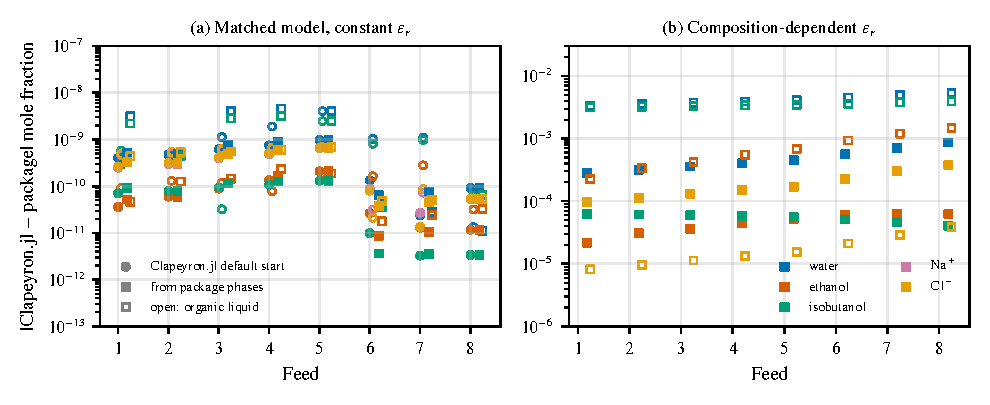
\includegraphics[width=\linewidth]{electrolyte-lle}
\caption{Matched and unmatched electrolyte code comparisons answer different questions (numerical verification).
(a) Constant-permittivity phase mole fractions agree below the $10^{-8}$ comparison line for both starts.
(b) Composition-dependent permittivity yields larger differences associated with the solvent Debye--H\"uckel derivative; the default comparator start returns no valid split.
Filled and open markers denote the water-rich and organic liquids, with the ionic fractions coincident by charge neutrality.
The model-convention and derivative probe is described in Supporting Information Section~\ref{sec:si-probe}.}
\label{fig:electrolyte-lle}
\end{figure}



\subsection{Derivative accuracy and reference resolution}
\label{sec:derivative-verification}
% P:verification-05
The 36 pressure-specified residual enthalpy, entropy and heat-capacity actions cover orders one to three for four electrolyte records, along declared temperature, pressure and composition directions.
Their criteria scale with the sum of the magnitudes of directional parts, preserving a meaningful scale when high-order terms cancel.
Every error is below 0.34 of its criterion (Fig.~\ref{fig:derivatives}a).
At third order the errors approach the estimated uncertainty of the refined references, so the observed agreement is reference-limited.
Independent implicit derivatives from Clapeyron.jl and FeOs test selected solved bubble-point and liquid--liquid responses separately from the package's own central differences (Fig.~\ref{fig:derivatives}b).

\begin{figure}[pos=H]
\centering
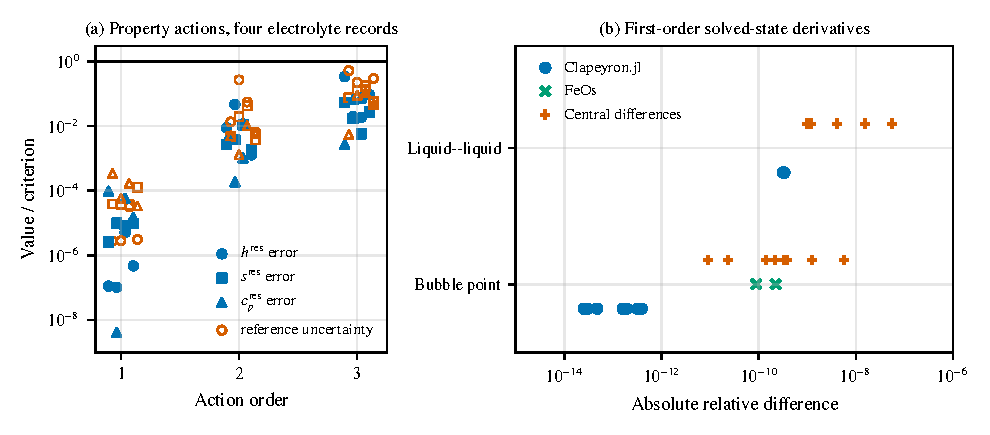
\includegraphics[width=\linewidth]{derivatives}
\caption{Derivative errors must be interpreted with the resolution of their references (numerical verification).
(a) Pressure-specified caloric-action errors divided by their criteria (filled), with refined-reference uncertainty on the same scale (open), grouped by order and parameter record.
(b) Selected first-order solved-state derivatives against independent implicit derivatives and the package's central differences.
Each point identifies an observable and physical direction; it is not an all-direction guarantee.}
\label{fig:derivatives}
\end{figure}

% P:verification-06
Second- and third-order solved actions use neutral ternary, single-phase electrolyte and manufactured reacting branches.
Refined lower-order actions and analytic isomerization values provide their references, with normalized errors shown in Table~\ref{tab:verification}.
Shared lower-order differentiation can conceal a common error and therefore does not replace the independent analytic comparisons.
The reacting caloric set contains 12\,975 comparisons, of which 122 have no numerical error-to-criterion ratio.
Among those with ratios the largest is 0.0952; all defining criteria are met.
Quadrature of equilibrium heat capacity and its temperature derivative recovers independently solved enthalpy and heat-capacity increments, providing a consistency check on the reference and reaction chains of Section~\ref{sec:derivatives}.
The chemistry is manufactured, so none of these counts is a calorimetric validation population.



\subsection{Balances, root selection and fitting calculations}
\label{sec:balances}
% P:verification-07
The density checks comprise 704 branch-specific requests evaluated in three modes, rather than three independent physical populations.
Selected densities agree with frozen references and a separate scan within the bounds in Table~\ref{tab:verification}, and reduced pressure residuals stay below $10^{-12}$.
The scan and selected-root routines share their equation evaluator.
Nested-grid agreement tests numerical root location on the finite searched domain, with no proof of complete enumeration.

% P:verification-07b
Given only the feed, temperature and pressure, explicit phase discovery returns the phases of the package's own declared solve for five neutral states: water/isobutanol with two liquids at 293.15~K and 100~kPa; water/ethanol/isobutanol with vapor and two liquids at 364.2~K and 100~kPa; single liquids of equimolar water/ethanol and of water with an isobutanol mole fraction of 0.005 at 293.15~K and 100~kPa; and a manufactured equimolar ternary with three liquids at 300~K and 10~MPa.
Across these states, the largest absolute composition difference is $1.94\times10^{-14}$, and the largest difference in $G/(RT)$, scaled by the larger of unity and the reference magnitude, is $7.67\times10^{-15}$.
For the equimolar water/hexane liquid at 300~K and 100~kPa (Fig.~\ref{fig:search-envelope}, top), the two stationary trials from near-pure liquid seeds agree with the FeOs stability analysis, and the discovered liquid split with the FeOs flash, within $1.58\times10^{-11}$ in mole fraction and $8.81\times10^{-11}$ in relative density after refinement of the FeOs results.
These are finite-point numerical comparisons, not physical validation or a global stability certificate.

% P:verification-07c
Charged trials check the condensed-phase condition of Section~\ref{sec:stability}: under a density-independent permittivity a charged trial point is admitted only as a mechanically stable density root on the liquid side of its own composition's pressure loop, and every seed and supplied point reported here returns the admission or unavailability that this condition predicts for it.
All four charged seeds are admitted for the water/ethanol/isobutanol/NaCl split at 293.15~K and 100~kPa, and both are admitted for the aqueous NaCl liquid at 298.15~K and 100~kPa.
For the reacting aqueous MEA/\ce{CO2} declarations at 318.15~K, a bubble at its solved pressure of 7.39816~kPa and a flash and a liquid at 5.9185286 and 8.8777929~kPa, three of four charged seeds are admitted; the remaining seed is unavailable because its only density root lies on the vapor side of its composition's pressure loop.
Trial points supplied by composition and density, rather than found by minimization, are admitted at the aqueous and salt-rich liquid roots of aqueous NaCl at 298.15~K and 100~kPa, whereas the aqueous vapor root, an off-root salt-rich point and a loop-less MEA point remain unavailable under the same condition, with no reported tangent-plane distance.
Unavailable points are never reclassified as stable because a distance could not be evaluated.
Among the reconstructed trial points, the largest normalization and charge defects are $2.64\times10^{-16}$ and $6.94\times10^{-18}$, both against a criterion of $10^{-12}$, and the largest difference between a trial's tangent-plane distance and the value implied by its balance multipliers, divided by $RT$, is $1.95\times10^{-13}$ against $10^{-10}$.
Discovery returns two liquids for the electrolyte split and one liquid each for the aqueous NaCl and reacting liquid declarations, the same phase counts as their declared solves.
For the MEA flash, whose declared two-phase solve succeeds, the search finds resolved descent but admits no declaration of lower Gibbs energy, so discovery stops explicitly without returning a phase set (Algorithm~\ref{alg:discovery}).
No discovery is requested for the free-pressure bubble.
These admission checks establish neither successful MEA flash discovery nor global stability; the estimated numerical uncertainty is not a rigorous bound.

% P:verification-08
A nine-species two-reaction lithium/sodium extraction declaration tests coupled balance and action calculations at 298.15~K and 101.325~kPa.
Over 67 central, perturbed and repeated solves, conserved-moiety defects are below $1.43\times10^{-14}$~mol and charge defects below $8.67\times10^{-15}$~mol.
The finer-step feed derivatives agree with exact actions within $3.52\times10^{-6}$ relative.
The pseudo-components and reaction constants are calibrated assumptions, so these results verify the declared numerical equations and supply no measured extraction accuracy.
The zero-inventory checks separately verify absent-species removal and allowed on-face calculations.
\todo{Insert numerical results for the reacting MEA flash family.}

% P:verification-09
Manufactured least-squares and minimax problems test known-parameter recovery and optimality equations, with the coordinate errors in Table~\ref{tab:verification}.
The electrolyte column comparison tests the full chain through density, reference and held Born diameter, rather than differentiating the final residual formula alone.
These checks establish numerical behavior on their declared observations; they do not imply identified physical ion parameters.
The process examples in Section~\ref{sec:applications} then test transport of the same native values and derivatives into an external equation-oriented model.
